\subsection{Метрики оценивания}\label{subsec:estimation_metrics}

\subsubsection{Регресионные метрики}
Точность рекомендательных систем обычно рассчитывается по одной из двух метрик: среднеквадратратическая ошибка (RMSE) и средняя абсолютная ошибка (MAE).
Обе этих метрики хорошо подходят для этой задачи, так как легко интерпретируются.
Однако, в некоторых случаях одной из них может отдаваться предпочтение в зависимости от данных.

\vspace{1em}
\textbf{Mean Absolute Error}

Средняя абсолютная ошибка представляет собой сумму абсолютных разностей между прогнозами и фактическими значениями:
\begin{equation}\label{eq:mae}
MAE = \frac{1}{|R|} \sum_{u \in U , i \in I} |r_{ui} - \hat{r_{ui}}|
\end{equation}
Основная черта этой метрики состоит в том, что она не никак не реагирует на большую величину конкретных разностей, но даёт целостное представление о точности работы рекомендательной системы.

\vspace{1em}
\textbf{Root Mean Squared Error}

Среднеквадратическая ошибка усиливает вклад больших ошибок, будучи чувствительной к плохим предсказаниям:
\begin{equation}\label{eq:rmse}
RMSE = \sqrt{\frac{1}{|R|} \sum_{u \in U , i \in I} (r_{ui} - \hat{r_{ui}})^2}
\end{equation}
Также стоит заметить, что эта метрика по определению всегда не меньше MAE\@.

В~\cite{chai} утверждается, что MAE лучше описывает ошибки, имеющие равномерное распределение, в то время как RMSE --- ошибки, имеющие нормальное распределение.

\subsubsection{Метрики классификации}
На практике часто не стоит задача сделать все предсказания как можно ближе к действительности, но правильно выделить некоторое количество подходящих объектов.
Для этого удобно использовать F-меру и площадь под кривыми ошибок.

\vspace{1em}
\textbf{F-мера}

Обычно классы релевантных и нерелевантных объектов не равны между собой по количеству членов, поэтому на каждом из классов имеет смысл ввести свою метрику, а затем объединить их в агрегированный критерий качества.
Для этого используются точность (precision) --- доля положительно классифицированных объектов, являющихся релевантными, от всех положительно классифицированных объектов и полнота (recall) --- доля положительно классифицированных объектов, являющихся релевантными, от всех релевантных объектов.
\begin{equation}\label{eq:precision}
precision = \frac{TP}{TP + FP}
\end{equation}
\begin{equation}\label{eq:recall}
recall = \frac{TP}{TP + FN}
\end{equation}

\vspace{1em}
В таблице~\ref{tab:conf_matrix} представлена так называемая матрица ошибок (confusion matrix), демонстрирующая смысл приведённых обозначений:

\begin{table}[h]
\centering
    \begin{tabular}{|P{2cm}|P{5cm}|P{5cm}|}
    \hline
    & $y = 1$ & $y = 0$\\ 
    \hline
    $\hat{y} = 1$ & True Positive (TP) & False Positive (FP)\\ 
    \hline
   $\hat{y} = 0$ & False Negative (FN) & True Negative (TN)\\
    \hline
    \end{tabular}
    \caption{Confusion Matrix}
    \label{tab:conf_matrix}
\end{table}


Полнота и точность агрегируются в F-меру с параметром $\beta$, определяющим вклад точности в оценку:

\begin{equation}\label{eq:f-metric}
F_\beta = (1 + \beta^2) \frac{precision\cdot recall}{\beta^2\cdot precision + recall}
\end{equation}

\pagebreak
\textbf{AUC-ROC и AUC-PR}

Вещественные алгоритмы используют пороговое значение для определения принадлежности объекта к какому-либо классу, однако привязка метрики к конкретному порогу не является оптимальным решением.
Оценить работу алгоритма в общем позволяет площадь под кривой ошибок (Area Under Curve).
ROC-кривая строится по координатам True Positive Rate (TPR) и False Positive Rate (FPR), соответствующих определённому значению порога.
\begin{equation}\label{eq:tpr}
TPR = \frac{TP}{TP + FN},
\end{equation}
\begin{equation}\label{eq:fpr}
FPR = \frac{FP}{FP + TN},
\end{equation}
где TPR --- полнота, FPR --- доля неверно классифицированных объектов класса нерелевантных объектов.
PR-кривая аналогично строится по координатам precision и recall.
Примеры кривых приведены ниже на рисунках~\ref{fig:roc_curve_example},~\ref{fig:pr_curve_example}:
\begin{figure}[h!]
\centering
\begin{minipage}{.5\textwidth}
\centering
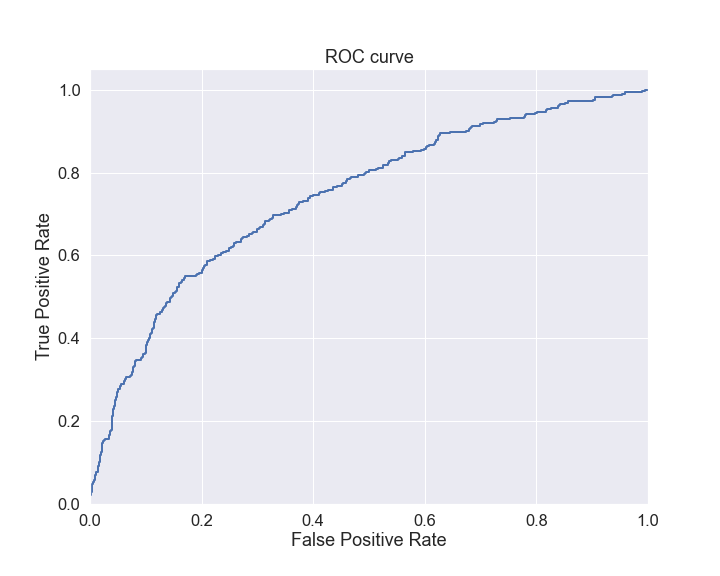
\includegraphics[width=1.1\linewidth]{images/roc_curve_example}
\caption{График ROC-кривой}
\label{fig:roc_curve_example}
\end{minipage}%
\begin{minipage}{.5\textwidth}
\centering
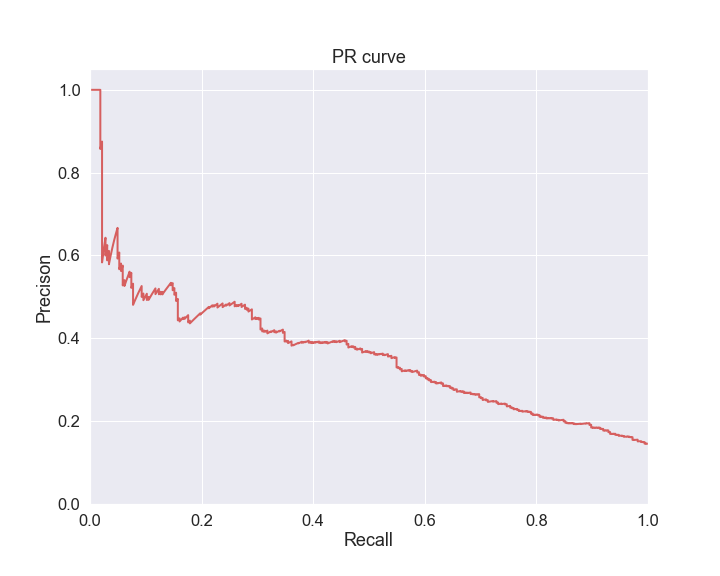
\includegraphics[width=1.1\linewidth]{images/pr_curve_example}
\caption{График PR-кривой}
\label{fig:pr_curve_example}
\end{minipage}
\end{figure}

Каждая точка на графике соответствует конкретному пороговому значению.
Чем больше площадь под кривой, тем выше качество классификации.


\subsubsection{Метрики качества ранжирования}
Зачастую может быть недостаточно предсказать оценку, которую пользователь поставит объекту, или то, окажется ли объект полезным.
В таком случае перед рекомендательной системой ставится задача ранжирования.
Задача ранжирования заключается в том, чтобы отсортировать набор элементов исходя из их релевенатности по отношению к пользователю.
В таком случае рекомендательный алгоритм помогают оценить метрики ранжирования.

Задача ранжирования может быть сформулирована следующим образом.
Рассмотрим множество пользователей $U = \{u_i\}_{i=1}^{N}$ и множество объектов $V = \{v_j\}_{j=1}^{M}$.
Результатом работы рекомендательного алгоритма является отображение $r_i: V \to \mathbb{R}$, присваивающее каждому объекту вес относительно конкретного пользователя.
Конечный набор весов задаёт для каждого пользователя перестановку $\{n_1, \dots, n_M\}$.
Для оценки качества необходимо иметь знание о степени релевантности ранжируемых объектов $\hat{r}_i$ - отображение, задающее перестановку $\{\hat{n}_1, \dots, \hat{n}_M\}$.
Истинное знание о релевантности может быть получено как за счёт имеющихся данных, так и на основе экспертной оценки.

\vspace{1em}
\textbf{Cumulative Gain(CG)}

CG представляет собой сумму истинных весов для $p$ релевантных объектов:
\begin{equation}\label{eq:cg}
CG_p = \sum_{j=1}^{p}\hat{r}_{n_j},
\end{equation}
где $\hat{r}_{n_j}$ --- истинная степень релевантности объекта на позиции $n_j$.

У метрики есть существенный недостаток - она нечувствительна к изменению порядка внутри $p$ релевантных объектов.

\vspace{1em}
\textbf{Discounted Cumulative Gain (DCG)}

DCG задаётся как~\cite{dcg}:
\begin{equation}\label{eq:dcg}
DCG_p = \sum_{j=1}^{p}\frac{\hat{r}_{n_j}}{\log_2 (j + 1)},
\end{equation}
где $\hat{r}_{n_j}$ --- истинная степень релевантности объекта на позиции $n_j$.

За счёт знаменателя метрика учитывает порядок объектов в списке.
Выбор логарифма в качестве функции дисконтирования обусловлен тем, что порядок объектов в начале списка важнее, чем в конце.
Теоретическое обоснование было дано в~\cite{dcg-log}.
Не хватает только нормализации, чтобы давать сравнимые значения для пользователей с разным количество рекомендаций.

\vspace{1em}
\textbf{Normalized Discounted Cumulative Gain (NDCG)}

Чтобы приобрести устойчивость к количеству элементов в списке - $p$, достаточно посчитать DCG для идеально отранжированного списка:
\begin{equation}\label{eq:ndcg}
NDCG_p = \frac{DCG_p}{IDCG_p},
\end{equation}
где IDCG - DCG для идеально отранжированного списка:
\begin{equation}\label{eq:idcg}
IDCG_p = \sum_{j=1}^{p}\frac{\hat{r}_{\hat{n}_j}}{\log_2 (j + 1)}
\end{equation}
Значение метрики всегда будет лежать в сегменте $[0,1]$.


\pagebreak
\subsection{Сравнение алгоритмов}\label{subsec:algos_comparison}
Каждая из моделей была обучена с полученными оптимальными гиперпараметрами.
В данном параграфе приводится оценка качества алгоритмов.
%Точность оценивается с помощью среднеквадратической ошибки и F1-меры.

Отдельного внимания заслуживают метрики классификации.
В задаче классификации определяются два класса объектов.
Вероятность принадлежности объекта $j$ к положительному классу рассчитывается следующим образом:
\begin{equation}
p_{ij} =
\begin{cases}
    0.5 + 0.5 \frac{\hat{r}_{ij} - \hat{r}_{i}^{\mean}}{\hat{r}_{i}^{\max} - \hat{r}_{i}^{\mean}}, & \hat{r}_{ij} - \hat{r}_{i}^{\mean} >= 0 \\
    0.5 - 0.5 \frac{\hat{r}_{ij} - \hat{r}_{i}^{\mean}}{\hat{r}_{i}^{\min} - \hat{r}_{i}^{\mean}}, & \hat{r}_{ij} - \hat{r}_{i}^{\mean} < 0
\end{cases}\label{eq:class_proba},
\end{equation}
где
$\hat{r}_{ij}$ --- предсказанная оценка, \\
$\hat{r}_{i}^{\mean}$, $\hat{r}_{i}^{\min}$, $\hat{r}_{i}^{\max}$ --- средняя, минимальная и максимальная предсказанные оценки пользователя.

На тестовом множестве считается, что объект относится к положительному классу, если пользователь поставил ему оценку выше своей средней.
%Для определённости в задаче классификации принято, что пользователь считает фильм плохим, если предсказанная оценка меньше его средней, и хорошим в обратном случае.

\subsubsection{Memory-based}
Схожесть будет рассчитываться с помощью центрированного косинусного сходства:

\begin{equation}
    sim(u, v) = \frac
    {\sum_{i \in I_u \cup I_v}{(r_{ui} - \bar r_u)(r_{vi} - \bar r_v)}}
    {\sqrt{\sum_{i \in I_u \cup I_v}{(r_{ui} - \bar r_u)^2}} 
    \sqrt{\sum_{i \in I_u \cup I_v}{(r_{vi} - \bar r_v)^2}}},\label{eq:equation2}
\end{equation}

Предсказанная оценка вычисляется с использованием взвешивания оценок похожих пользователей и стандартизированной оценки:
\begin{equation}
    r_{ui} = \bar r_u + \sigma_u \frac
    {\sum_{u' \in U_u}{sim(u, u')\frac{(r_{u'i} - \bar r_{u'})}{\sigma_{u'}}}}
    {\sum_{u' \in U_u}{sim(u, u')}}\label{eq:equation3}
\end{equation}

%\pagebreak
Совместим user-based и item-based подходы, определяя вклад каждого из них с помощью параметра $\alpha$.
К чистым user-based и item-based алгоритмам относятся значения $\alpha = 0$ и $\alpha = 1$ соответственно:

\begin{equation}\label{eq:memory_hybrid}
r_{ui} = (1 - \alpha)\space UB(u, i) + \alpha\space IB(u,i)
\end{equation}

Оценка качества алгоритма представлена в таблице~\ref{tab:memory_based_quality}:
\vspace{1em}
\begin{table}[h]
    \resizebox{\textwidth}{!}{%
    \begin{tabular}{ |P{4.5em}|P{2.5em}|P{2.5em}|P{2.5em}|P{2.5em}|P{2.5em}|P{2.5em}|P{2.5em}|P{2.5em}|P{2.5em}|P{2.5em}|P{2.5em}|}
    \hline
    $\alpha$ & 0 & 0.1 & 0.2 & 0.3 & 0.4 & 0.5 & 0.6 & 0.7 & 0.8 & 0.9 & 1\\
    \hline
    RMSE & 0.8847 & 0.8732 & 0.8635 & 0.8560 & 0.8504 & 0.8471 & \cellcolor{green!45}0.8458 & 0.8468 & 0.8498 & 0.8551 & 0.8624 \\
    \hline
    MAE & 0.6619 & 0.6540 & 0.6473 & 0.6420 & 0.6381 & 0.6356 & \cellcolor{green!45}0.6347 & 0.6353 & 0.6376 & 0.6415 & 0.6470 \\
    \hline
    NDCG & 0.9576 & 0.9583 & 0.9593 & 0.9601 & 0.9602 & \cellcolor{green!45}0.9607 & 0.9607 & 0.9603 & 0.9598 & 0.9592 & 0.9587 \\
    \hline
    F1 & 0.7172 & 0.7197 & 0.7224 & 0.7241 & 0.7254 & 0.7253 & 0.7257 & \cellcolor{green!45}0.7259 & 0.7239 & 0.7213 & 0.7199 \\
    \hline
    AUC-ROC & 0.7079 & 0.7126 & 0.7158 & 0.7181 & 0.7196 & 0.7207 & \cellcolor{green!45}0.7211 & 0.7202 & 0.7185 & 0.7157 & 0.7122 \\
    \hline
    AUC-PR & 0.7307 & 0.7358 & 0.7388 & 0.7406 & 0.7421 & 0.7433 & \cellcolor{green!45}0.7436 & 0.7417 & 0.7388 & 0.7353 & 0.7310 \\
    \hline
    \end{tabular}}
    \caption{Значения метрик в зависимости от $\alpha$}
    \label{tab:memory_based_quality}
\end{table}

Графики кривых при $\alpha = 0.6$ представлены на рисунках~\ref{fig:memory_based_roc},~\ref{fig:memory_based_pr}:

\begin{figure}[h!]
\centering
\begin{minipage}{.5\textwidth}
\centering
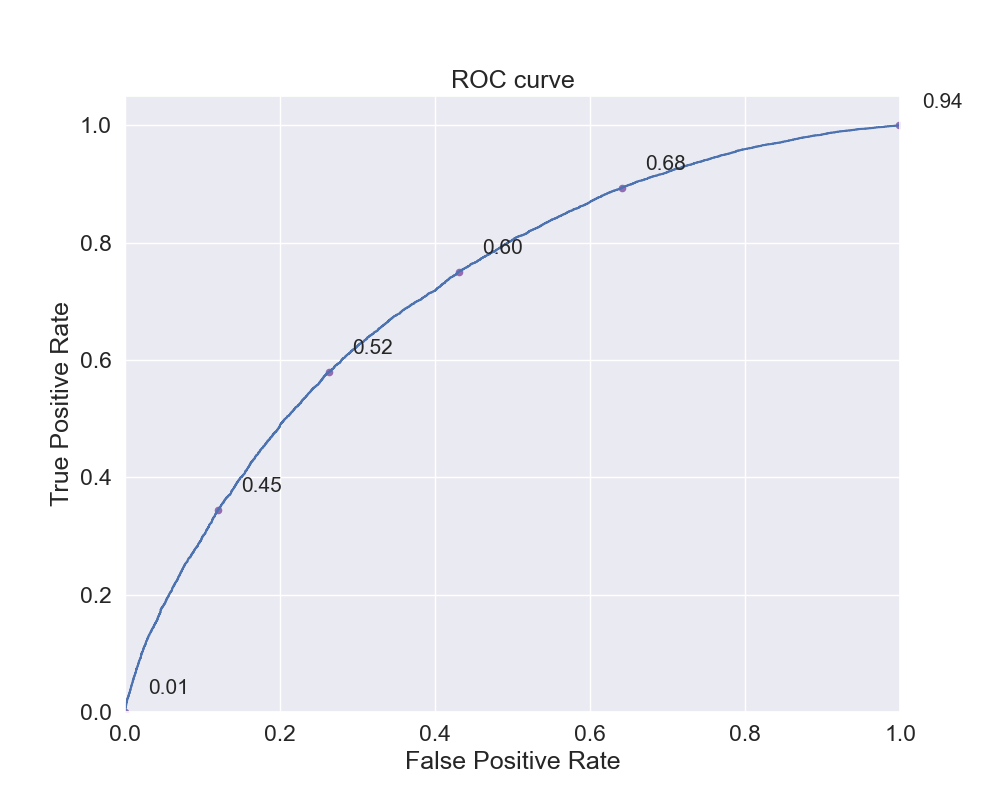
\includegraphics[width=1.1\linewidth]{images/mixed_memory_based/roc_curve}
\caption{График ROC-кривой}
\label{fig:memory_based_roc}
\end{minipage}%
\begin{minipage}{.5\textwidth}
\centering
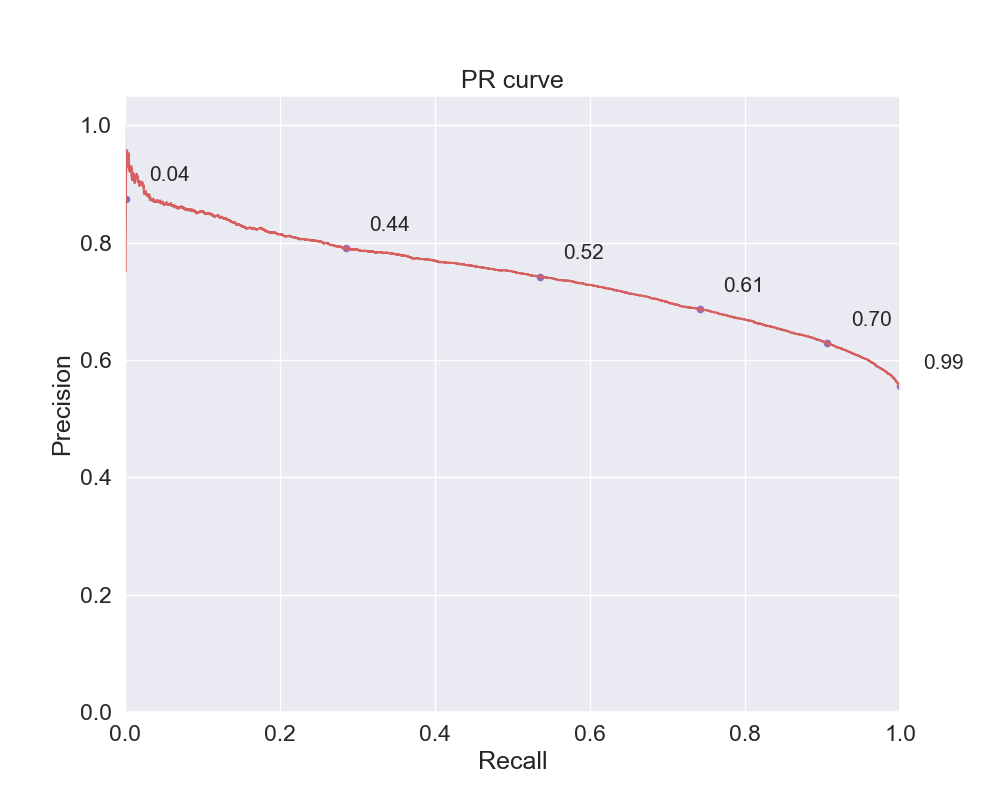
\includegraphics[width=1.1\linewidth]{images/mixed_memory_based/pr_curve}
\caption{График PR-кривой}
\label{fig:memory_based_pr}
\end{minipage}
\end{figure}

\pagebreak

\subsubsection{Model-based}
\vspace{1em}
\textbf{Alternating Least Squares}

Оценка качества представлена в таблице~\ref{tab:als_quality}:

\begin{table}[h]
    \centering{
    \begin{tabular}{ |P{4.8em}|P{4.8em}|P{4.8em}|P{4.8em}|P{4.8em}|P{4.8em}|}
    \hline
    RMSE & MAE & NDCG & F1 & AUC-ROC & AUC-PR \\
    \hline
    0.8754 & 0.6802 & 0.9609 & 0.7296 & 0.7040 & 0.7268 \\
    \hline
    \end{tabular}}
    \caption{Значения метрик для ALS}
    \label{tab:als_quality}
\end{table}

Графики ROC/PR-кривых приведены на рисунках~\ref{fig:als_roc},~\ref{fig:als_pr}:

\begin{figure}[h!]
\centering
\begin{minipage}{.5\textwidth}
\centering
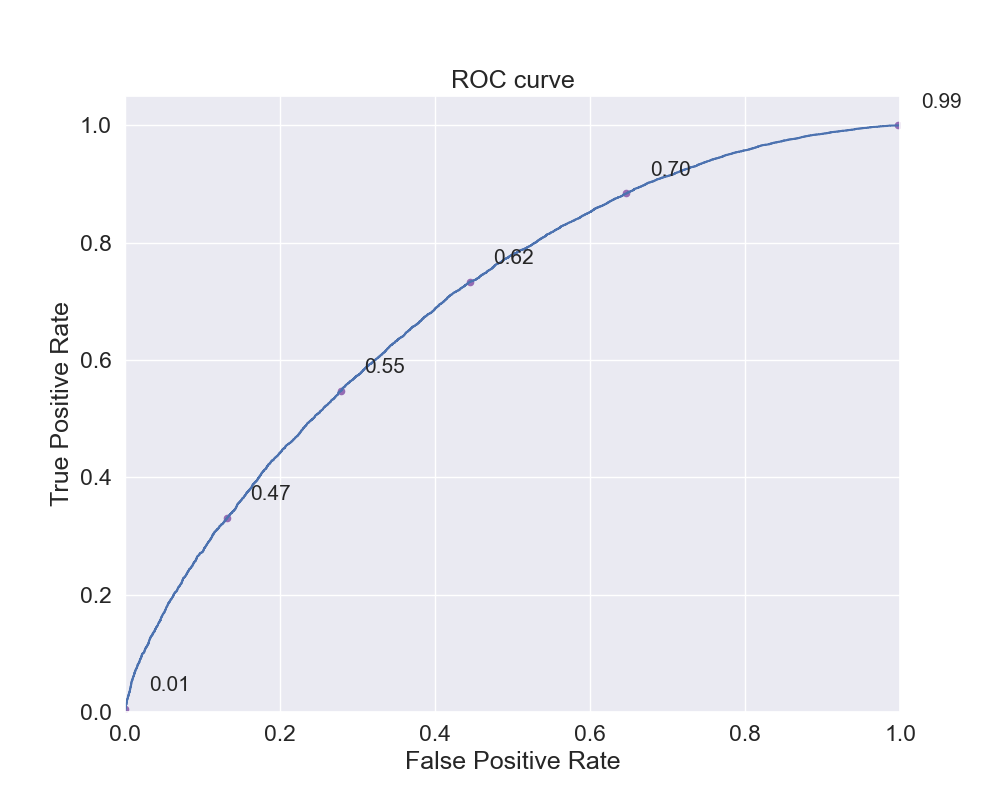
\includegraphics[width=0.9\linewidth]{images/als/roc_curve}
\caption{График ROC-кривой для ALS}
\label{fig:als_roc}
\end{minipage}%
\begin{minipage}{.5\textwidth}
\centering
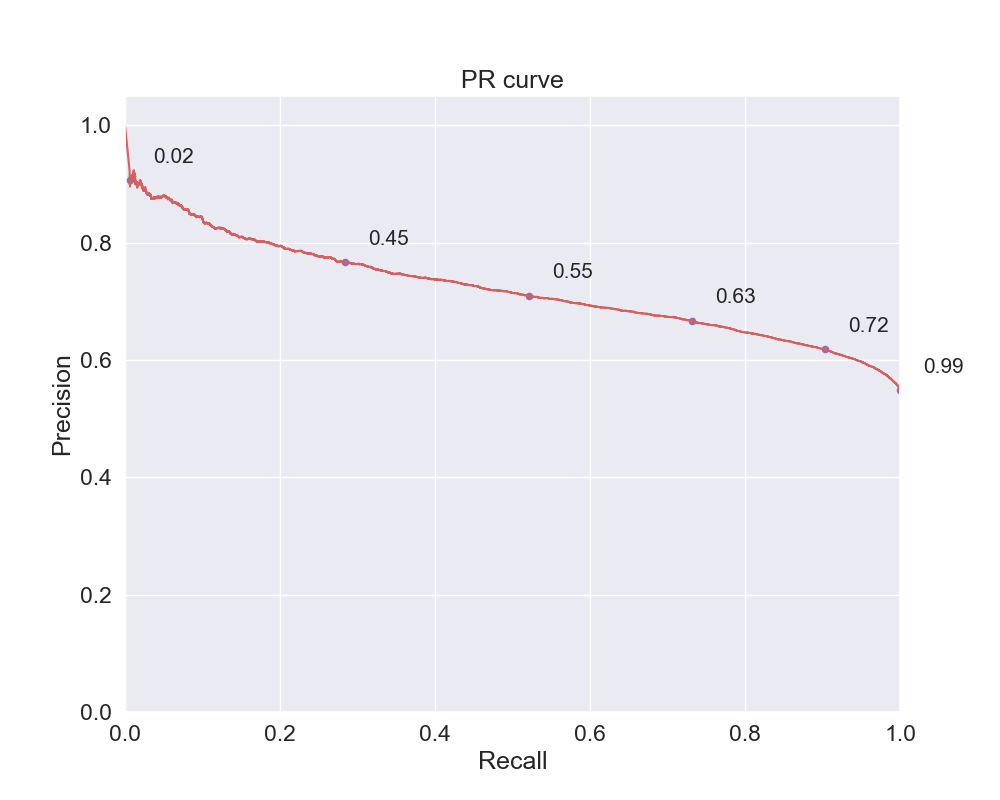
\includegraphics[width=0.9\linewidth]{images/als/pr_curve}
\caption{График PR-кривой для ALS}
\label{fig:als_pr}
\end{minipage}
\end{figure}

Значения метрик в процессе обучения представлены на рисунках~\ref{fig:als_real_losses},~\ref{fig:als_class_losses}:

\begin{figure}[h!]
\centering
\begin{minipage}{.5\textwidth}
\centering
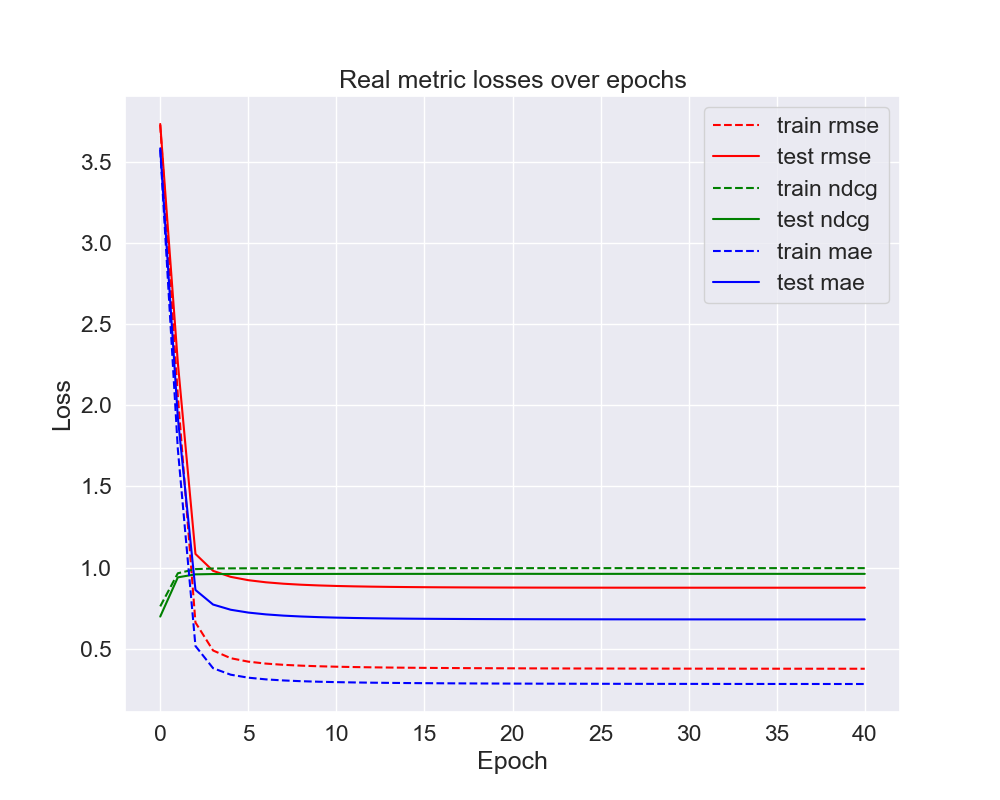
\includegraphics[width=0.9\linewidth]{images/als/real_losses}
\caption{Регрессионные метрики ALS}
\label{fig:als_real_losses}
\end{minipage}%
\begin{minipage}{.5\textwidth}
\centering
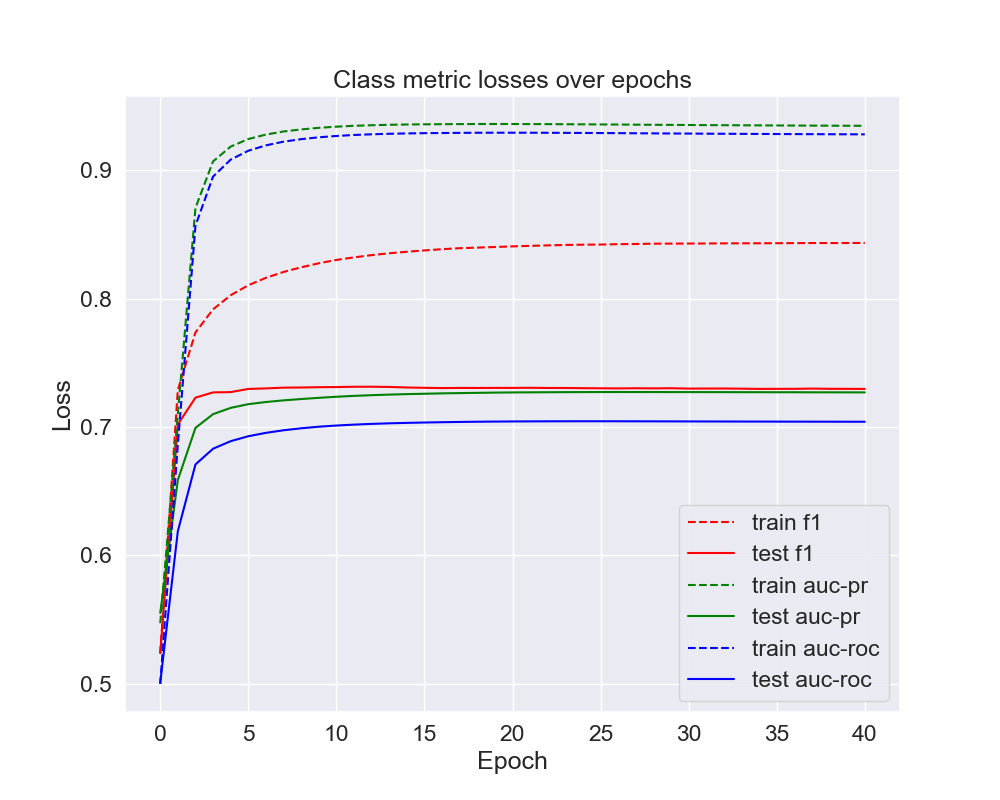
\includegraphics[width=0.9\linewidth]{images/als/class_losses}
\caption{Метрики классификации ALS}
\label{fig:als_class_losses}
\end{minipage}
\end{figure}


\vspace{1em}
\textbf{Stochastic Gradient Descent}

Оценка качества представлена в таблице~\ref{tab:sgd_quality}:

\begin{table}[h]
    \centering{
    \begin{tabular}{ |P{4.8em}|P{4.8em}|P{4.8em}|P{4.8em}|P{4.8em}|P{4.8em}|}
    \hline
    RMSE & MAE & NDCG & F1 & AUC-ROC & AUC-PR \\
    \hline
    0.8357 & 0.6373 & 0.9616 & 0.7287 & 0.7221 & 0.7428 \\
    \hline
    \end{tabular}}
    \caption{Значения метрик для SGD}
    \label{tab:sgd_quality}
\end{table}

Графики ROC/PR-кривых приведены на рисунках~\ref{fig:sgd_roc},~\ref{fig:sgd_pr}:

\begin{figure}[h!]
\centering
\begin{minipage}{.5\textwidth}
\centering
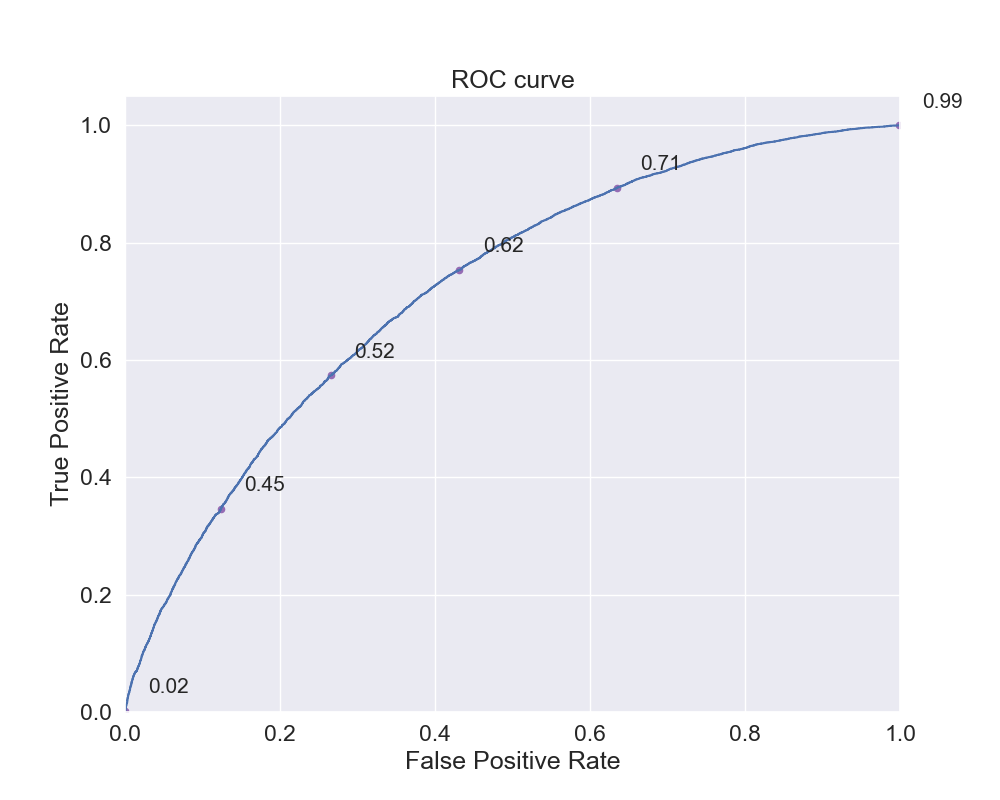
\includegraphics[width=1.0\linewidth]{images/sgd/roc_curve}
\caption{График ROC-кривой для SGD}
\label{fig:sgd_roc}
\end{minipage}%
\begin{minipage}{.5\textwidth}
\centering
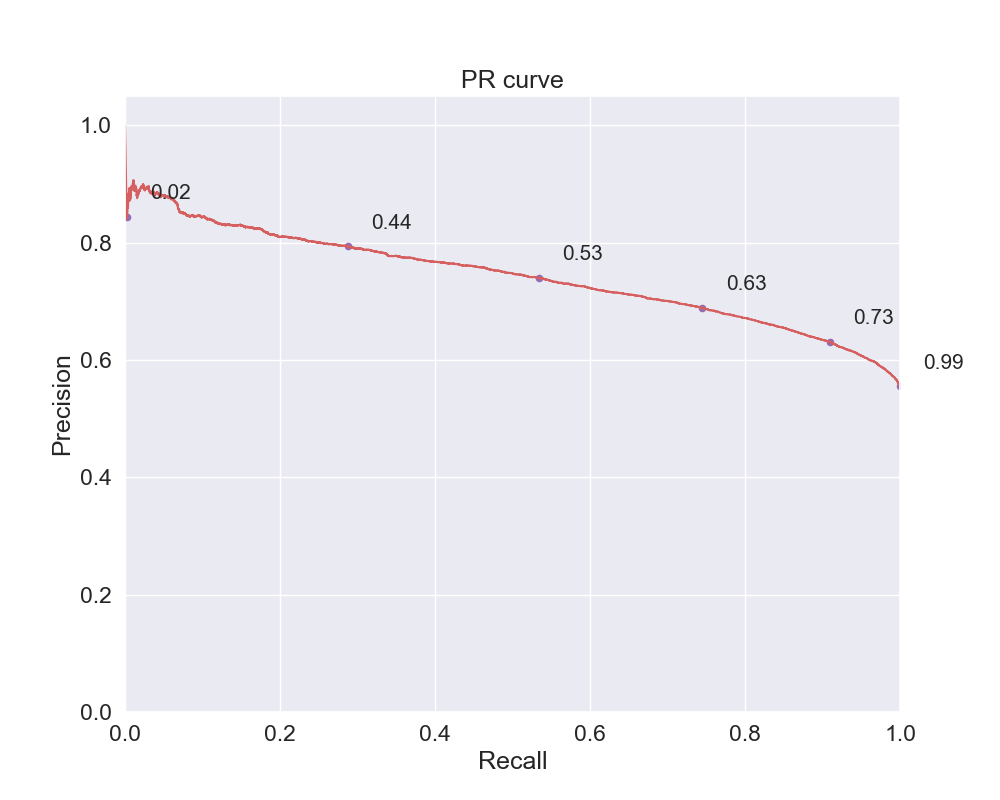
\includegraphics[width=1.0\linewidth]{images/sgd/pr_curve}
\caption{График PR-кривой для SGD}
\label{fig:sgd_pr}
\end{minipage}
\end{figure}

Значения метрик в процессе обучения представлены на рисунках~\ref{fig:sgd_real_losses},~\ref{fig:sgd_class_losses}:

\begin{figure}[h!]
\centering
\begin{minipage}{.5\textwidth}
\centering
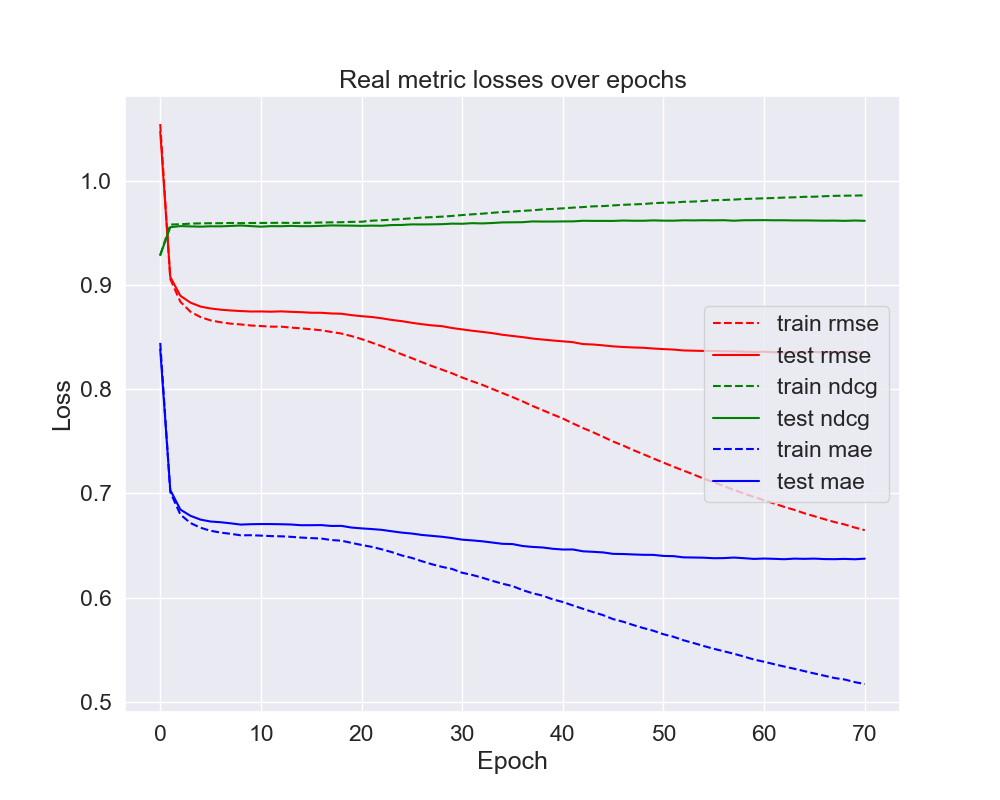
\includegraphics[width=1.0\linewidth]{images/sgd/real_losses}
\caption{Регрессионные метрики SGD}
\label{fig:sgd_real_losses}
\end{minipage}%
\begin{minipage}{.5\textwidth}
\centering
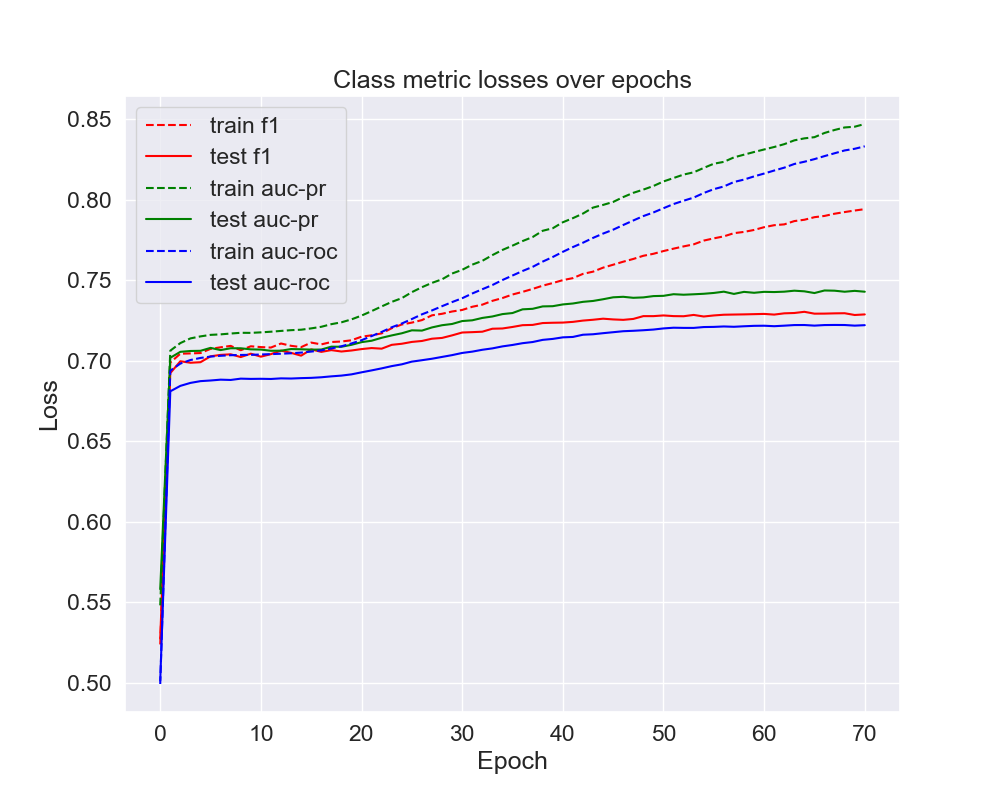
\includegraphics[width=1.0\linewidth]{images/sgd/class_losses}
\caption{Метрики классификации SGD}
\label{fig:sgd_class_losses}
\end{minipage}
\end{figure}

\pagebreak

\vspace{1em}
\textbf{Probabilistic Matrix Factorization}

Оптимизация функции потерь производилась посредством SGD\@.\\
Оценка качества представлена в таблице~\ref{tab:pmf_sgd_quality}:

\begin{table}[h]
    \centering{
    \begin{tabular}{ |P{4.8em}|P{4.8em}|P{4.8em}|P{4.8em}|P{4.8em}|P{4.8em}|}
    \hline
    RMSE & MAE & NDCG & F1 & AUC-ROC & AUC-PR \\
    \hline
    0.9135 & 0.7082 & 0.9554 & 0.7127 & 0.6780 & 0.7017 \\
    \hline
    \end{tabular}}
    \caption{Значения метрик для PMF}
    \label{tab:pmf_sgd_quality}
\end{table}

Графики ROC/PR-кривых приведены на рисунках~\ref{fig:pmf_sgd_roc},~\ref{fig:pmf_sgd_pr}:

\begin{figure}[h!]
\centering
\begin{minipage}{.5\textwidth}
\centering
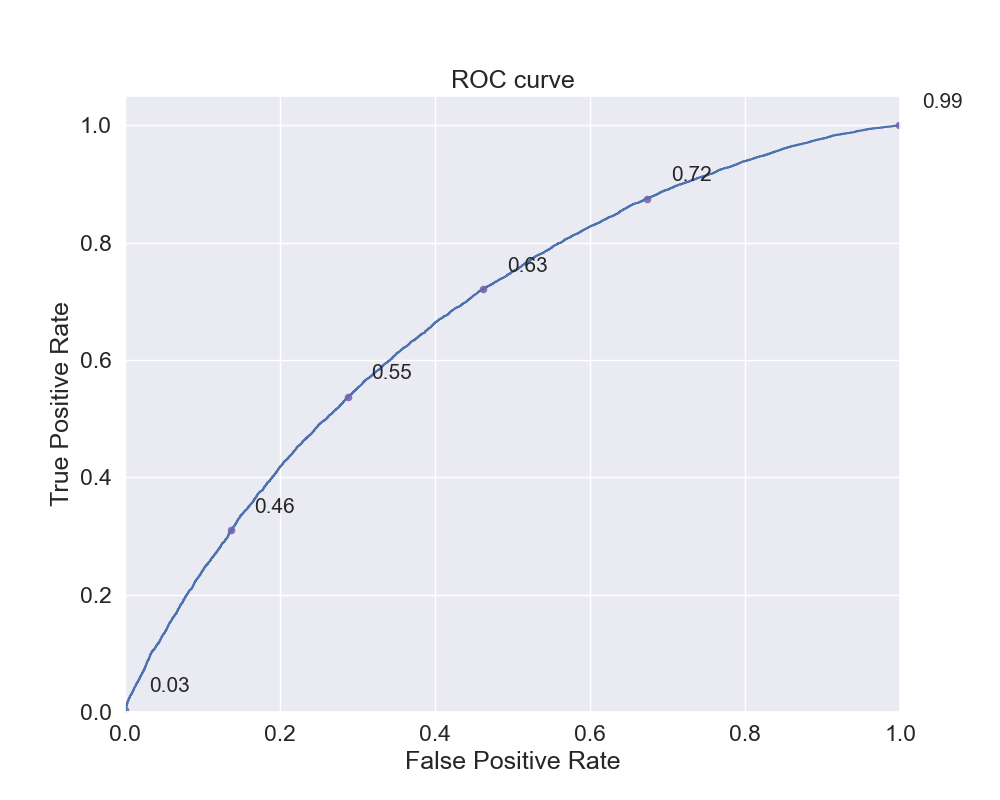
\includegraphics[width=1.0\linewidth]{images/pmf_sgd/roc_curve}
\caption{График ROC-кривой для PMF}
\label{fig:pmf_sgd_roc}
\end{minipage}%
\begin{minipage}{.5\textwidth}
\centering
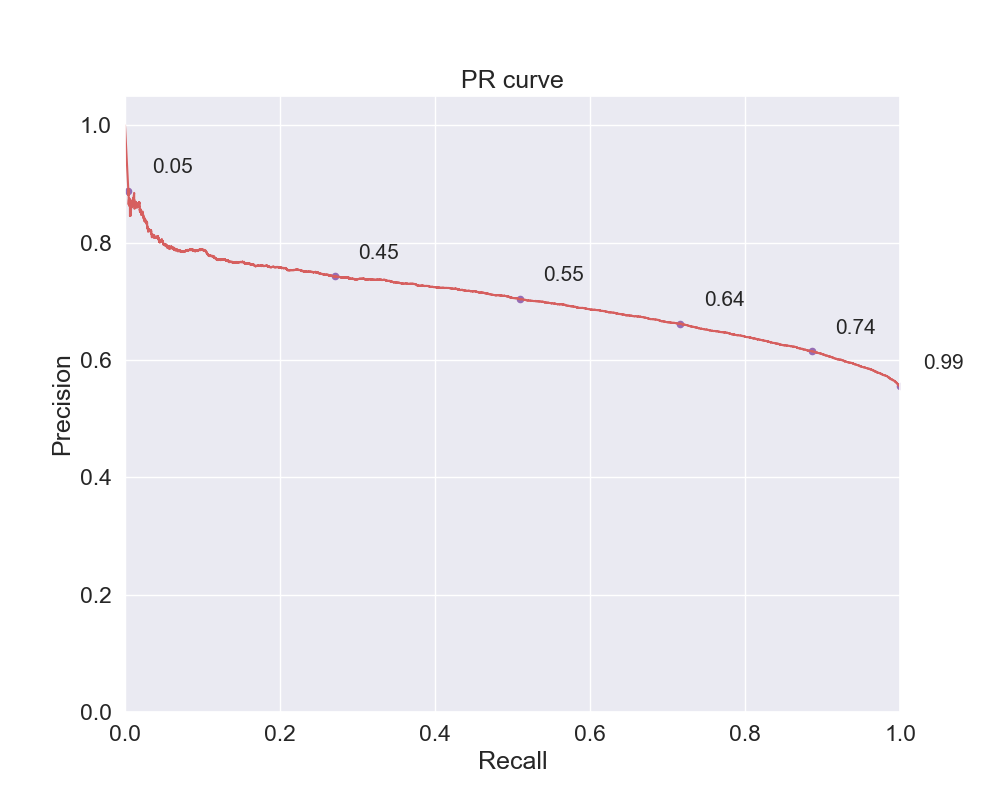
\includegraphics[width=1.0\linewidth]{images/pmf_sgd/pr_curve}
\caption{График PR-кривой для PMF}
\label{fig:pmf_sgd_pr}
\end{minipage}
\end{figure}

Значения метрик в процессе обучения представлены на рисунках~\ref{fig:pmf_sgd_real_losses},~\ref{fig:pmf_sgd_class_losses}:

\begin{figure}[h!]
\centering
\begin{minipage}{.5\textwidth}
\centering
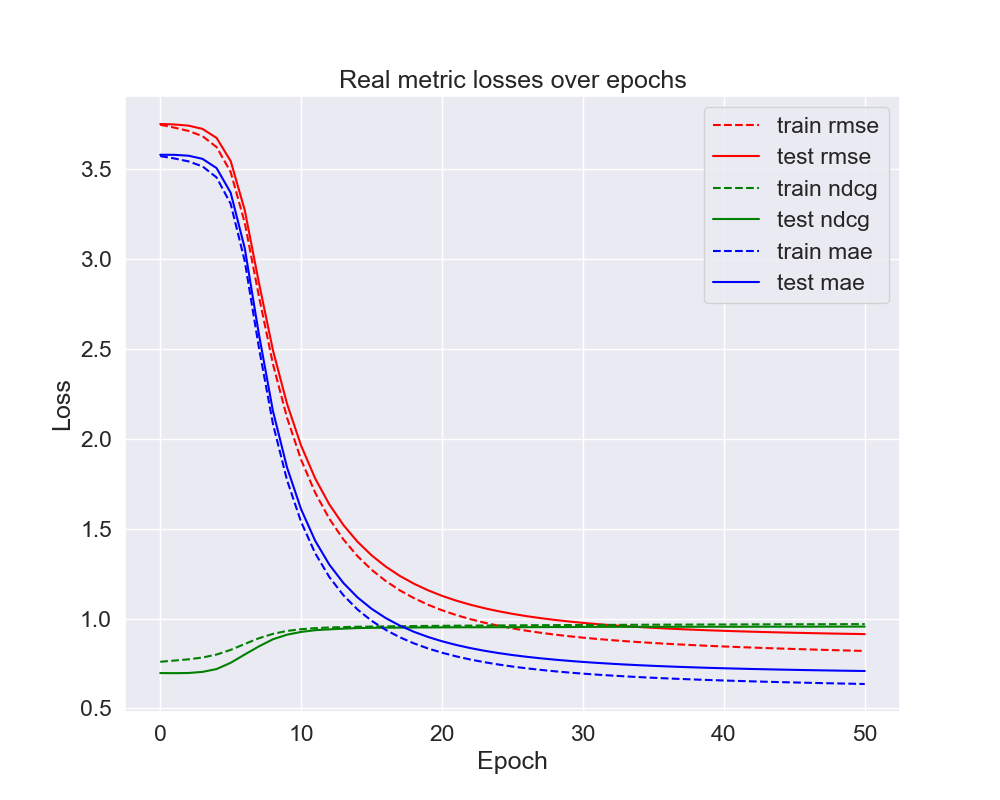
\includegraphics[width=1.0\linewidth]{images/pmf_sgd/real_losses}
\caption{Регрессионные метрики PMF}
\label{fig:pmf_sgd_real_losses}
\end{minipage}%
\begin{minipage}{.5\textwidth}
\centering
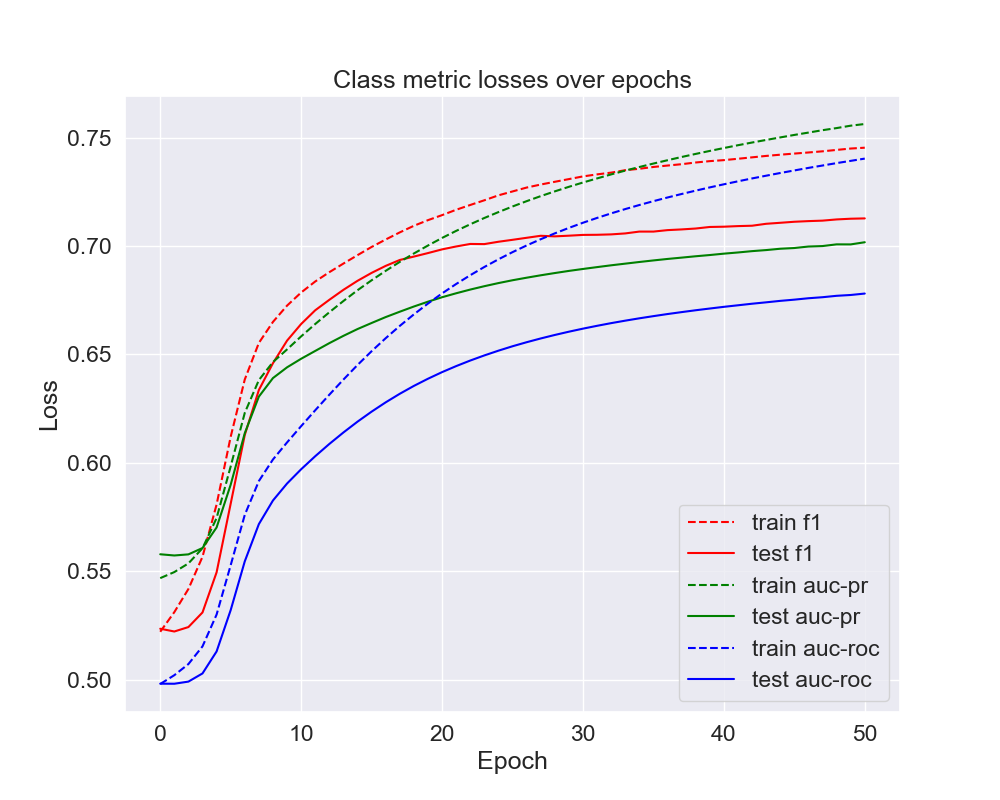
\includegraphics[width=1.0\linewidth]{images/pmf_sgd/class_losses}
\caption{Метрики классификации PMF}
\label{fig:pmf_sgd_class_losses}
\end{minipage}
\end{figure}


\vspace{1em}
\textbf{Neural Network}

Оценка качества представлена в таблице~\ref{tab:nn_quality}:

\begin{table}[h]
    \centering{
    \begin{tabular}{ |P{4.8em}|P{4.8em}|P{4.8em}|P{4.8em}|P{4.8em}|P{4.8em}|}
    \hline
    RMSE & MAE & NDCG & F1 & AUC-ROC & AUC-PR \\
    \hline
    0.8587 & 0.6532 & 0.9581 & 0.7130 & 0.7010 & 0.7227 \\
    \hline
    \end{tabular}}
    \caption{Значения метрик для нейросети}
    \label{tab:nn_quality}
\end{table}

Графики ROC/PR-кривых приведены на рисунках~\ref{fig:nn_roc},~\ref{fig:nn_pr}:

\begin{figure}[h!]
\centering
\begin{minipage}{.5\textwidth}
\centering
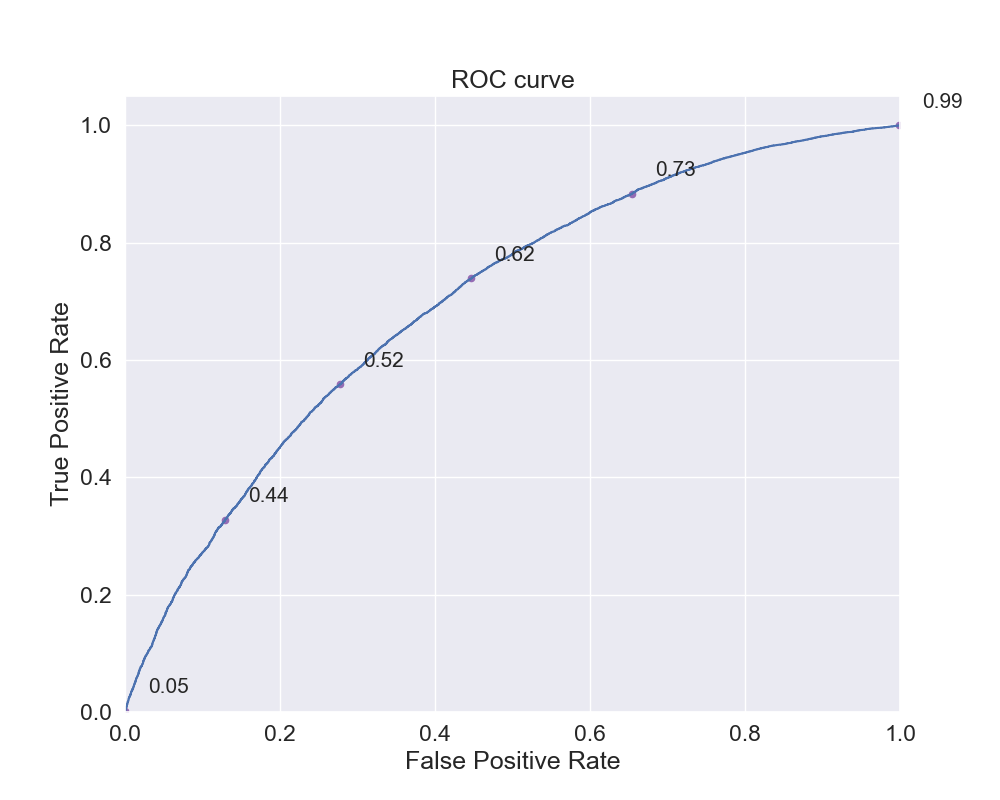
\includegraphics[width=1.0\linewidth]{images/neural_net/roc_curve}
\caption{График ROC-кривой нейросети}
\label{fig:nn_roc}
\end{minipage}%
\begin{minipage}{.5\textwidth}
\centering
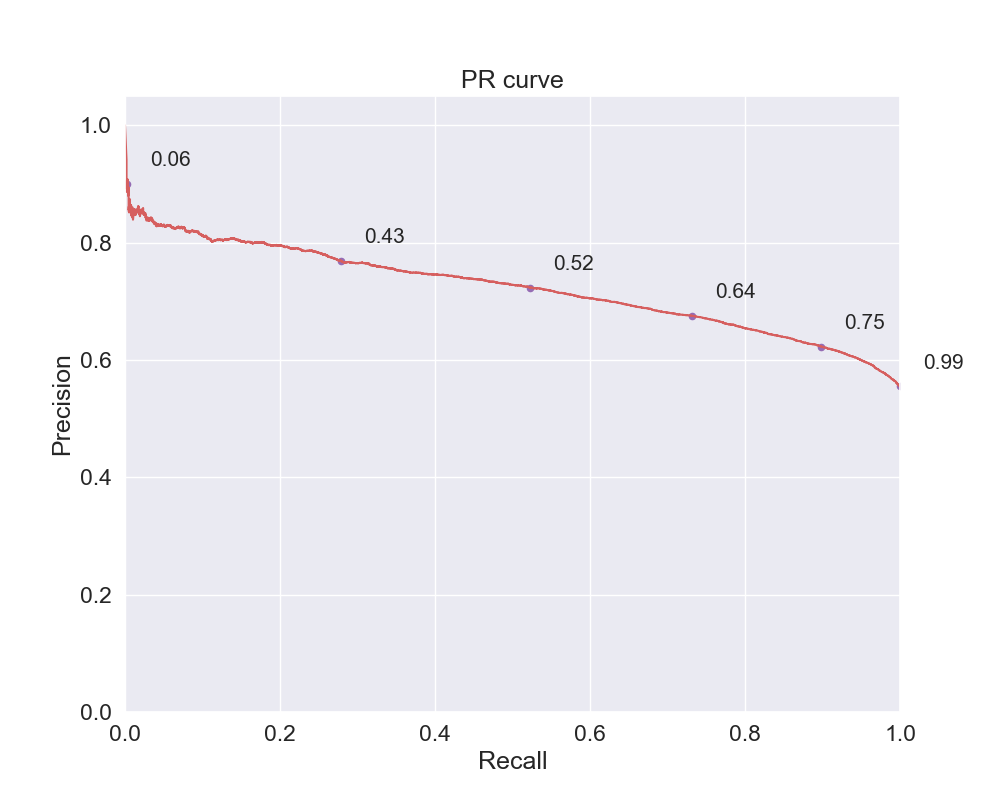
\includegraphics[width=1.0\linewidth]{images/neural_net/pr_curve}
\caption{График PR-кривой нейросети}
\label{fig:nn_pr}
\end{minipage}
\end{figure}

Значения метрик в процессе обучения представлены на рисунках~\ref{fig:nn_real_losses},~\ref{fig:nn_class_losses}:

\begin{figure}[h!]
\centering
\begin{minipage}{.5\textwidth}
\centering
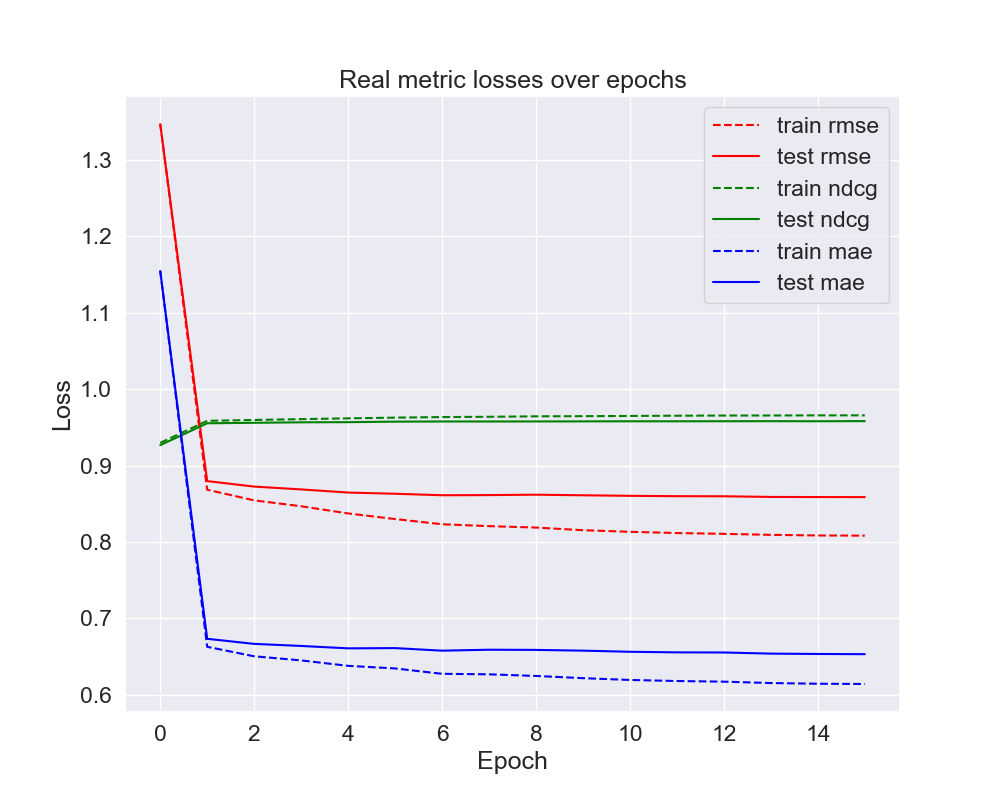
\includegraphics[width=1.0\linewidth]{images/neural_net/real_losses}
\caption{Регрессионные метрики}
\label{fig:nn_real_losses}
\end{minipage}%
\begin{minipage}{.5\textwidth}
\centering
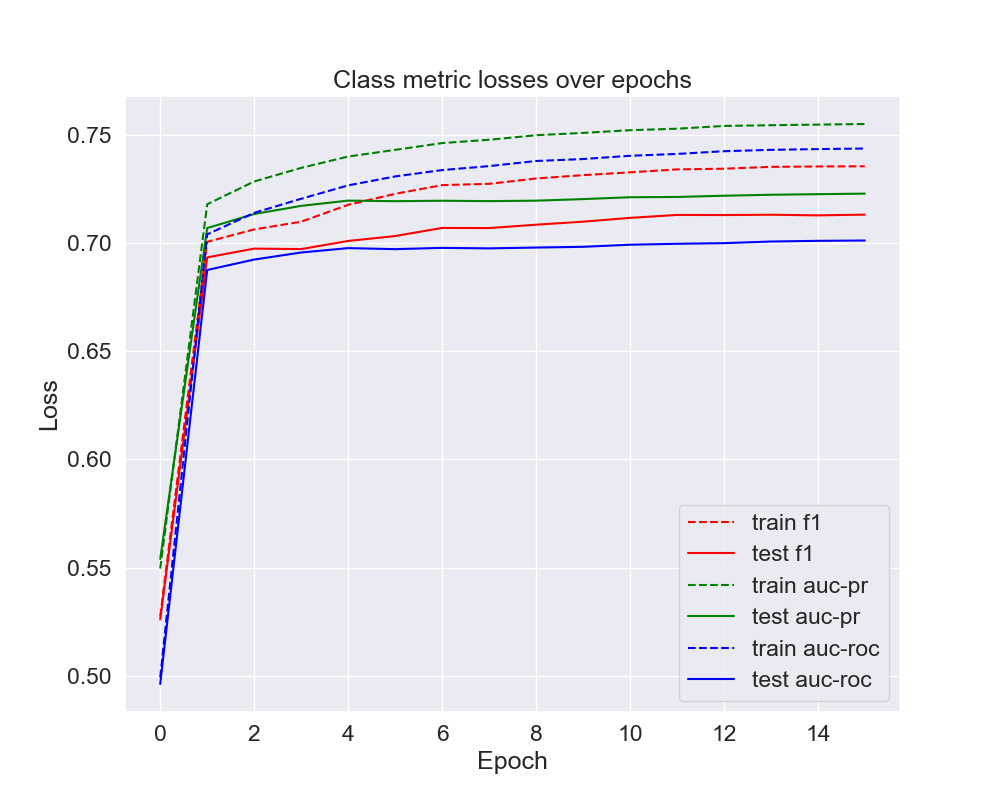
\includegraphics[width=1.0\linewidth]{images/neural_net/class_losses}
\caption{Метрики классификации}
\label{fig:nn_class_losses}
\end{minipage}
\end{figure}

\pagebreak

\subsubsection{Content-based}
Оценка качества представлена в таблице~\ref{tab:content_quality}:

\begin{table}[h]
    \centering{
    \begin{tabular}{ |P{4.8em}|P{4.8em}|P{4.8em}|P{4.8em}|P{4.8em}|P{4.8em}|}
    \hline
    RMSE & MAE & NDCG & F1 & AUC-ROC & AUC-PR \\
    \hline
    1.18735 & 0.8976 & 0.9449 & 0.6693 & 0.6037 & 0.6417 \\
    \hline
    \end{tabular}}
    \caption{Значения метрик}
    \label{tab:content_quality}
\end{table}

Графики ROC/PR-кривых приведены на рисунках~\ref{fig:content_roc},~\ref{fig:content_pr}:

\begin{figure}[h!]
\centering
\begin{minipage}{.5\textwidth}
\centering
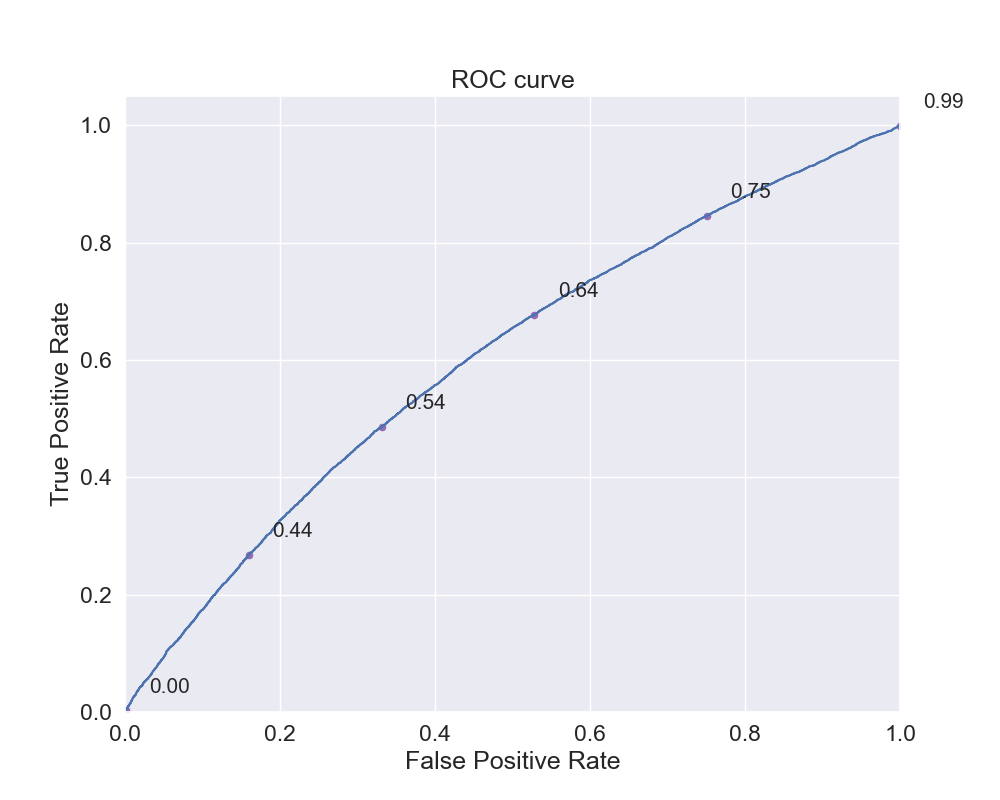
\includegraphics[width=0.9\linewidth]{images/content/roc_curve}
\caption{График ROC-кривой}
\label{fig:content_roc}
\end{minipage}%
\begin{minipage}{.5\textwidth}
\centering
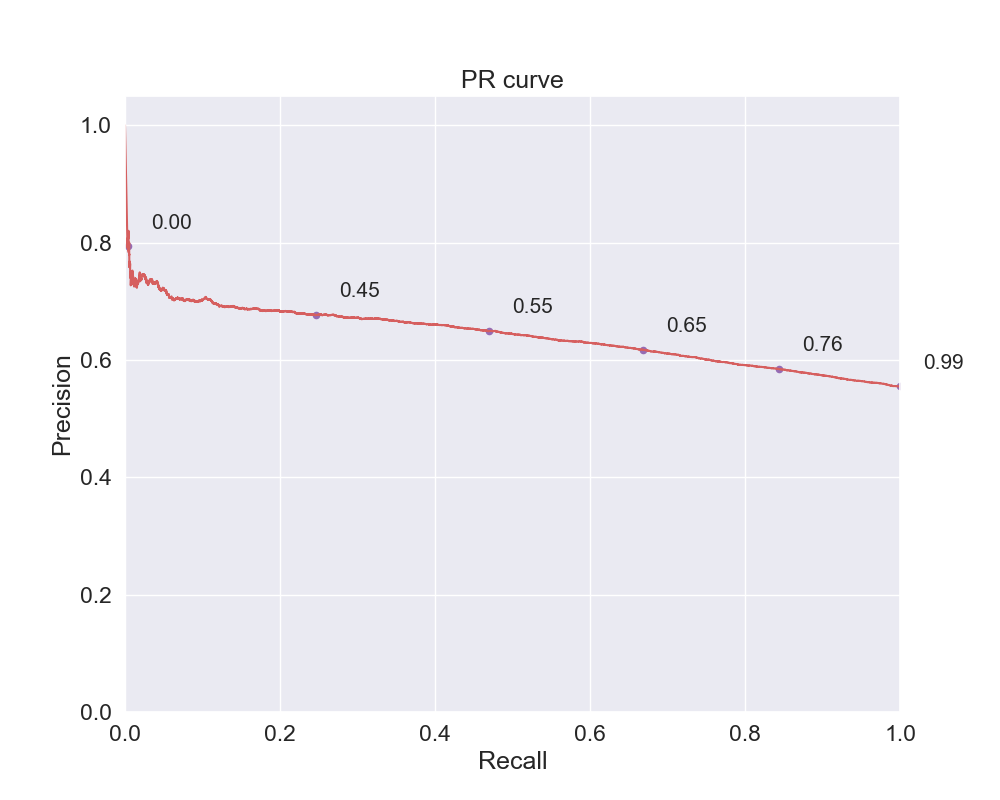
\includegraphics[width=0.9\linewidth]{images/content/pr_curve}
\caption{График PR-кривой}
\label{fig:content_pr}
\end{minipage}
\end{figure}

Среднеквадратическая ошибка автоэнкодера в процессе обучения представлена на рисунке~\ref{fig:autoencoder_losses}:

\begin{figure}[h!]
\centering
\begin{minipage}{0.6\textwidth}
\centering
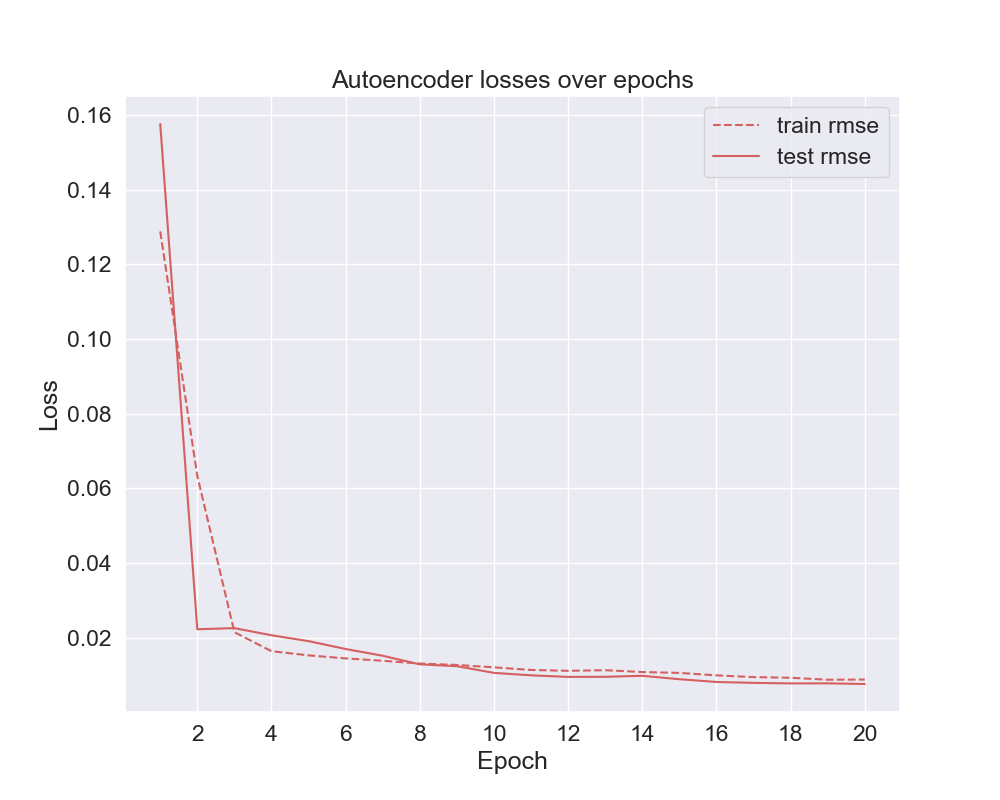
\includegraphics[width=0.85\linewidth]{images/content/autoencoder_losses}
\caption{Среднеквадратическая ошибка автоэнкодера}
\label{fig:autoencoder_losses}
\end{minipage}%
\end{figure}

\pagebreak

\subsubsection{Hybrid}
Для оценки гибридной модели в качестве коллаборативной модели использовалось SGD-разложение, а в качестве контентной - автоэнкодер, обученный сжимать tf-idf пространство тэгов.

Вклад каждой модели варьироваался посредством параметра $\alpha$.
К ответам чистых коллаборативной и контентной моделей относятся значения $\alpha = 0$ и $\alpha = 1$ соответственно:
\begin{equation}\label{eq:hybrid_filtering}
\hat{r}_{ij} = (1 - \alpha)\space SGD(i, j) + \alpha\space C(i, j)
\end{equation}

Оценка качества алгоритма представлена в таблице~\ref{tab:hybrid_quality}:
\vspace{1em}
\begin{table}[h]
    \resizebox{\textwidth}{!}{%
    \begin{tabular}{ |P{4.5em}|P{2.5em}|P{2.5em}|P{2.5em}|P{2.5em}|P{2.5em}|P{2.5em}|P{2.5em}|P{2.5em}|P{2.5em}|P{2.5em}|P{2.5em}|}
    \hline
    $\alpha$ & 0 & 0.1 & 0.2 & 0.3 & 0.4 & 0.5 & 0.6 & 0.7 & 0.8 & 0.9 & 1 \\
    \hline
    RMSE & \cellcolor{green!45}0.8357 & 0.8405 & 0.8535 & 0.8744 & 0.9026 & 0.9374 & 0.9782 & 1.0242 & 1.0748 & 1.1294 & 1.1873 \\
    \hline
    MAE & \cellcolor{green!45}0.6373 & 0.6383 & 0.6461 & 0.6599 & 0.6792 & 0.7040 & 0.7339 & 0.7685 & 0.8077 & 0.8510 & 0.8976 \\
    \hline
    NDCG & 0.9616 & 0.9619 & 0.9623 & \cellcolor{green!45}0.9625 & 0.9620 & 0.9613 & 0.9596 & 0.9581 & 0.9550 & 0.9503 & 0.9449 \\
    \hline
    F1 & 0.7287 & 0.7293 & 0.7312 & \cellcolor{green!45}0.7318 & 0.7315 & 0.7309 & 0.7268 & 0.7199 & 0.7093 & 0.6914 & 0.6693 \\
    \hline
    AUC-ROC & 0.7221 & 0.7233 & 0.7241 & \cellcolor{green!45}0.7242 & 0.7228 & 0.7190 & 0.7116 & 0.6983 & 0.6765 & 0.6443 & 0.6037 \\
    \hline
    AUC-PR & 0.7428 & 0.7439 & 0.7446 & \cellcolor{green!45}0.7446 & 0.7428 & 0.7384 & 0.7309 & 0.7192 & 0.7017 & 0.6754 & 0.6417 \\
    \hline
    \end{tabular}}
    \caption{Значения метрик в зависимости от $\alpha$}
    \label{tab:hybrid_quality}
\end{table}

Графики кривых при $\alpha = 0.3$ представлены на рисунках~\ref{fig:hybrid_roc},~\ref{fig:hybrid_pr}:

\begin{figure}[h!]
\centering
\begin{minipage}{.5\textwidth}
\centering
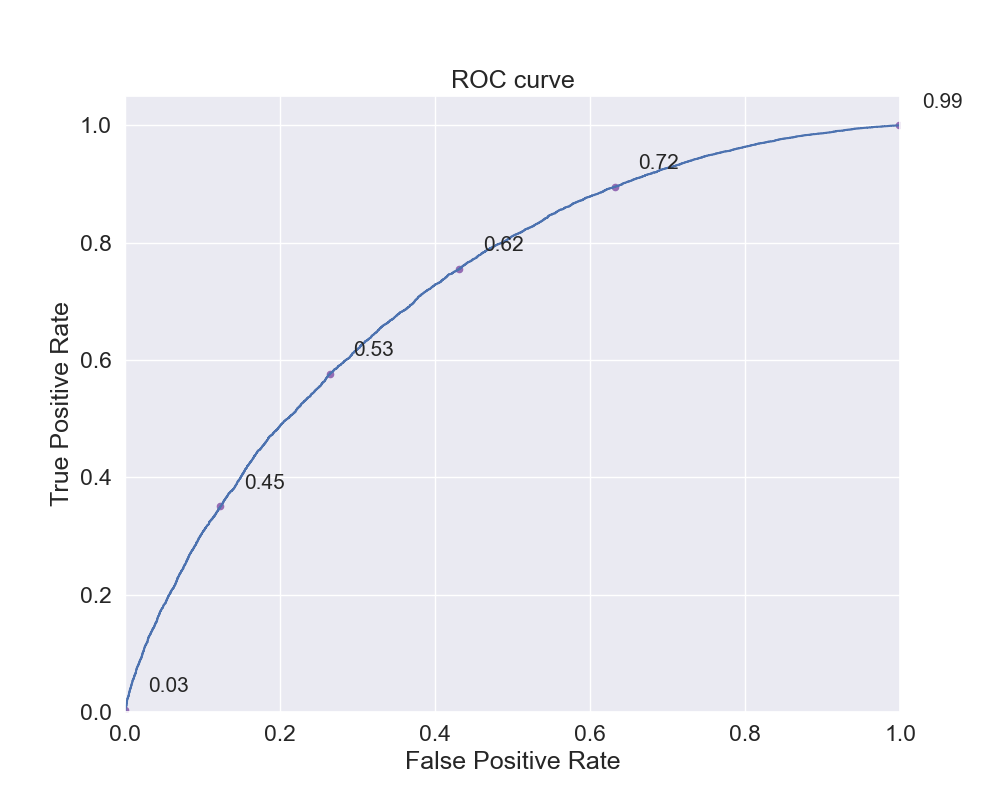
\includegraphics[width=1.1\linewidth]{images/hybrid/roc_curve}
\caption{График ROC-кривой}
\label{fig:hybrid_roc}
\end{minipage}%
\begin{minipage}{.5\textwidth}
\centering
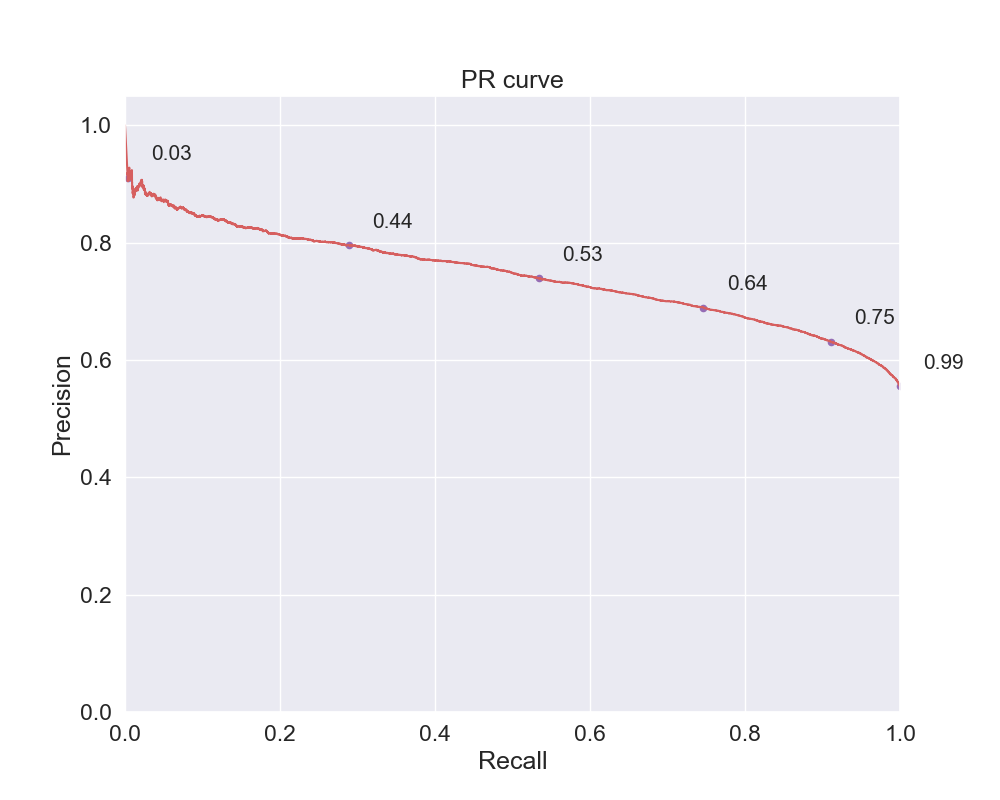
\includegraphics[width=1.1\linewidth]{images/hybrid/pr_curve}
\caption{График PR-кривой}
\label{fig:hybrid_pr}
\end{minipage}
\end{figure}

\pagebreak